\documentclass{article}

\usepackage{graphicx}
\usepackage{subfigure}
\usepackage[hypcap]{caption}
\usepackage{listings}
\usepackage{float}
\floatstyle{plaintop}
\restylefloat{table}

\title{Experimental Design and Data Analysis: Assignment 4}
\author{Andrew Bedard(2566978) \& Simone van Gompel(2567525) \\ Group 19}

\begin{document}

  \maketitle

  \section*{Exercise 1}
    \subsection*{1}
    \subsection*{2}
    \subsection*{3}
    \subsection*{4}
    
  \section*{Exercise 2}
    \subsection*{1}
      \begin{figure}[H]
          \centering
          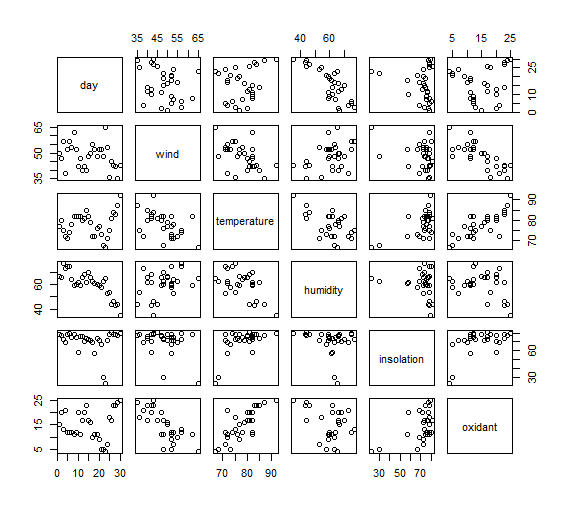
\includegraphics[scale=0.6]{../results/2_1.png}
          \caption{Pairplot of the airpollution data}
          \label{fig:BoxHours}
      \end{figure} 
    \subsection*{2}
      \begin{figure}[H]
          \centering
          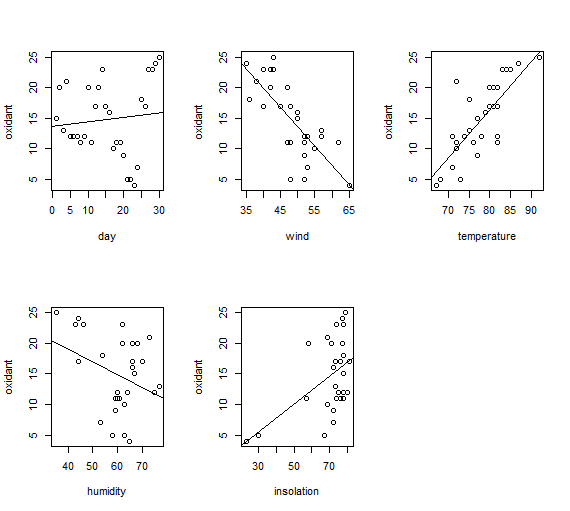
\includegraphics[scale=0.6]{../results/2_2.png}
          \caption{The linear regression of the explanatory variables}
          \label{fig:BoxHours}
      \end{figure} 
    \subsection*{3}
    \subsection*{4}
    \subsection*{5}

  \section*{Exercise 3}
    \subsection*{1}
    \subsection*{2}
    \subsection*{3}
    \subsection*{4}
    \subsection*{5}

  \section*{Exercise 4}
    
  \section{R-Code}
    \subsection{Exercise 1}\label{sec:RE1}
      \begin{lstlisting}[language=R]
      \end{lstlisting}
    \subsection{Exercise 2}\label{sec:RE2}
      \begin{lstlisting}[language=R]
      \end{lstlisting}
    \subsection{Exercise 3}\label{sec:RE3}
      \begin{lstlisting}[language=R]
      \end{lstlisting}
    \subsection{Exercise 4}\label{sec:RE4}
      \begin{lstlisting}[language=R]
      \end{lstlisting}
\end{document}
